\section{Simulations for Stationary Strategies}
\begin{figure}[h]
    \centering
    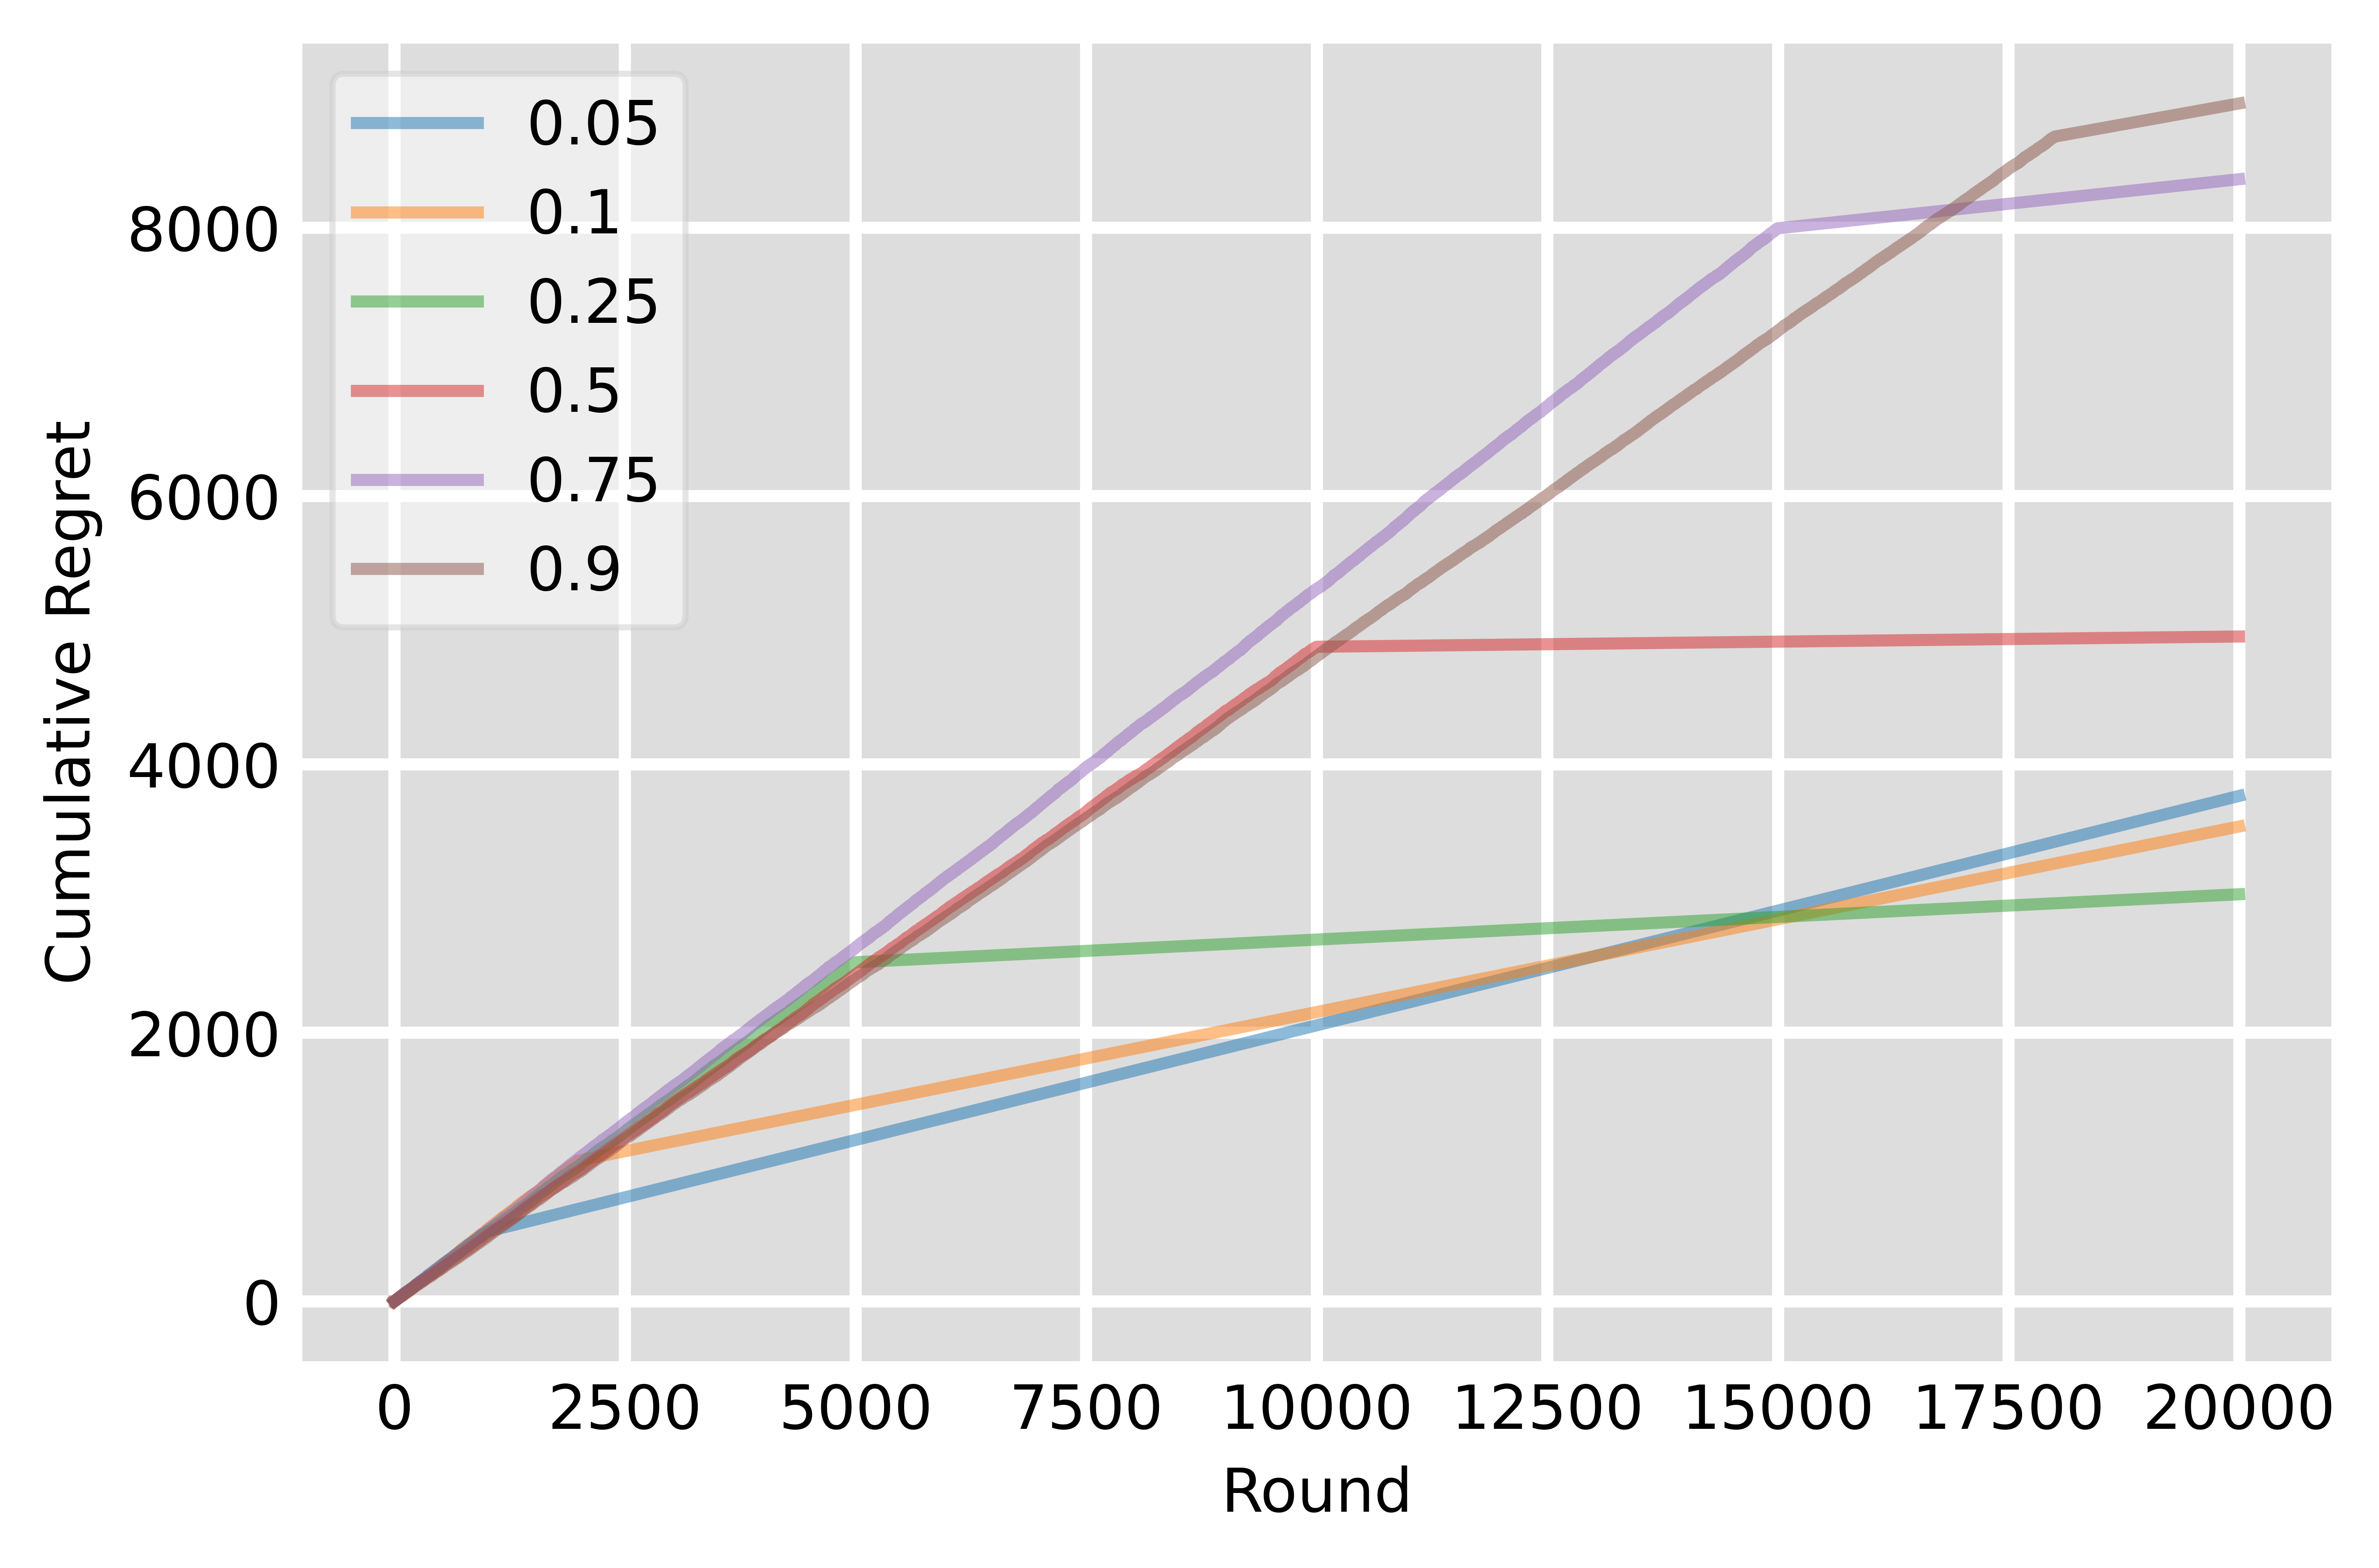
\includegraphics[width=0.9\textwidth]{figures/epsilon_plot.png}
    \caption[Epsilon-first strategy with varying values of epsilon]{Epsilon-first strategy with varying values of epsilon. 100 machines. 20000 rounds per iteration. Average of 50 iterations}
    \label{fig: epsilon}
\end{figure}

\begin{figure}[h]
    \centering
    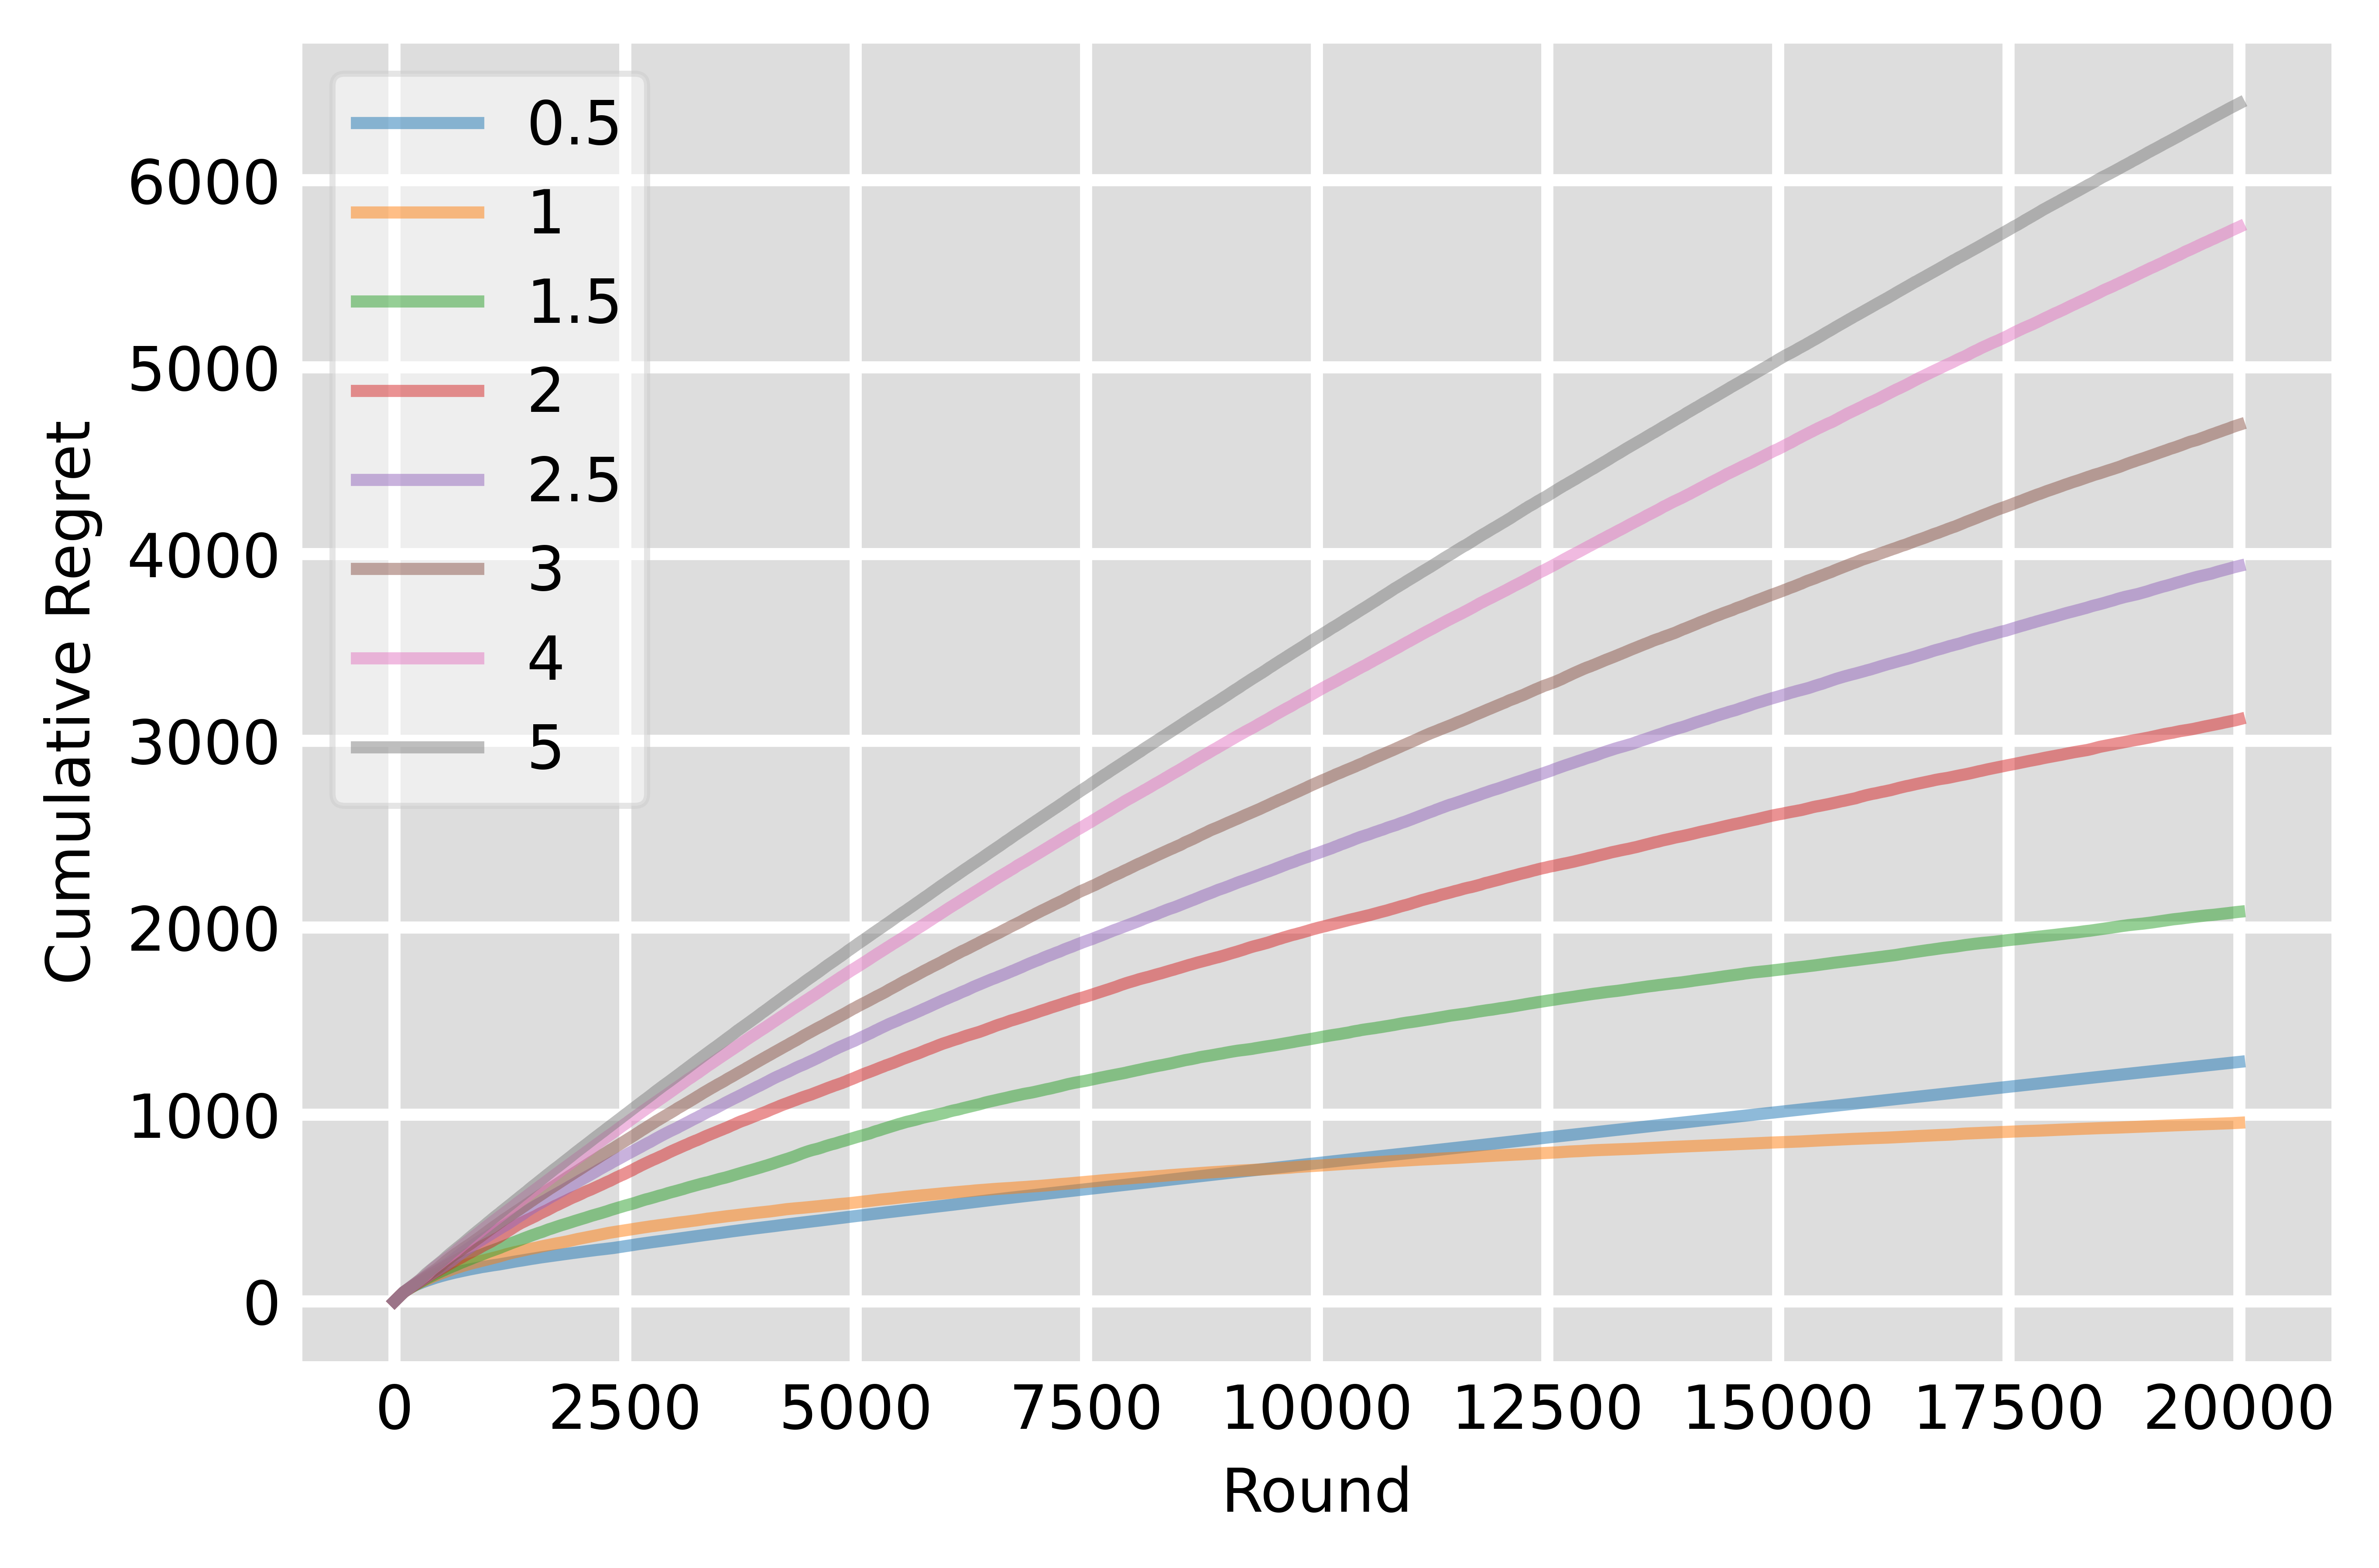
\includegraphics[width=0.9\textwidth]{figures/ucb_plot.png}
    \caption[UCB strategy with varying values of confidence level]{UCB strategy with varying values of confidence level. 100 machines. 20000 rounds per iteration. Average of 50 iterations}
    \label{fig: ucb}
\end{figure}

\begin{figure}[h]
    \centering
    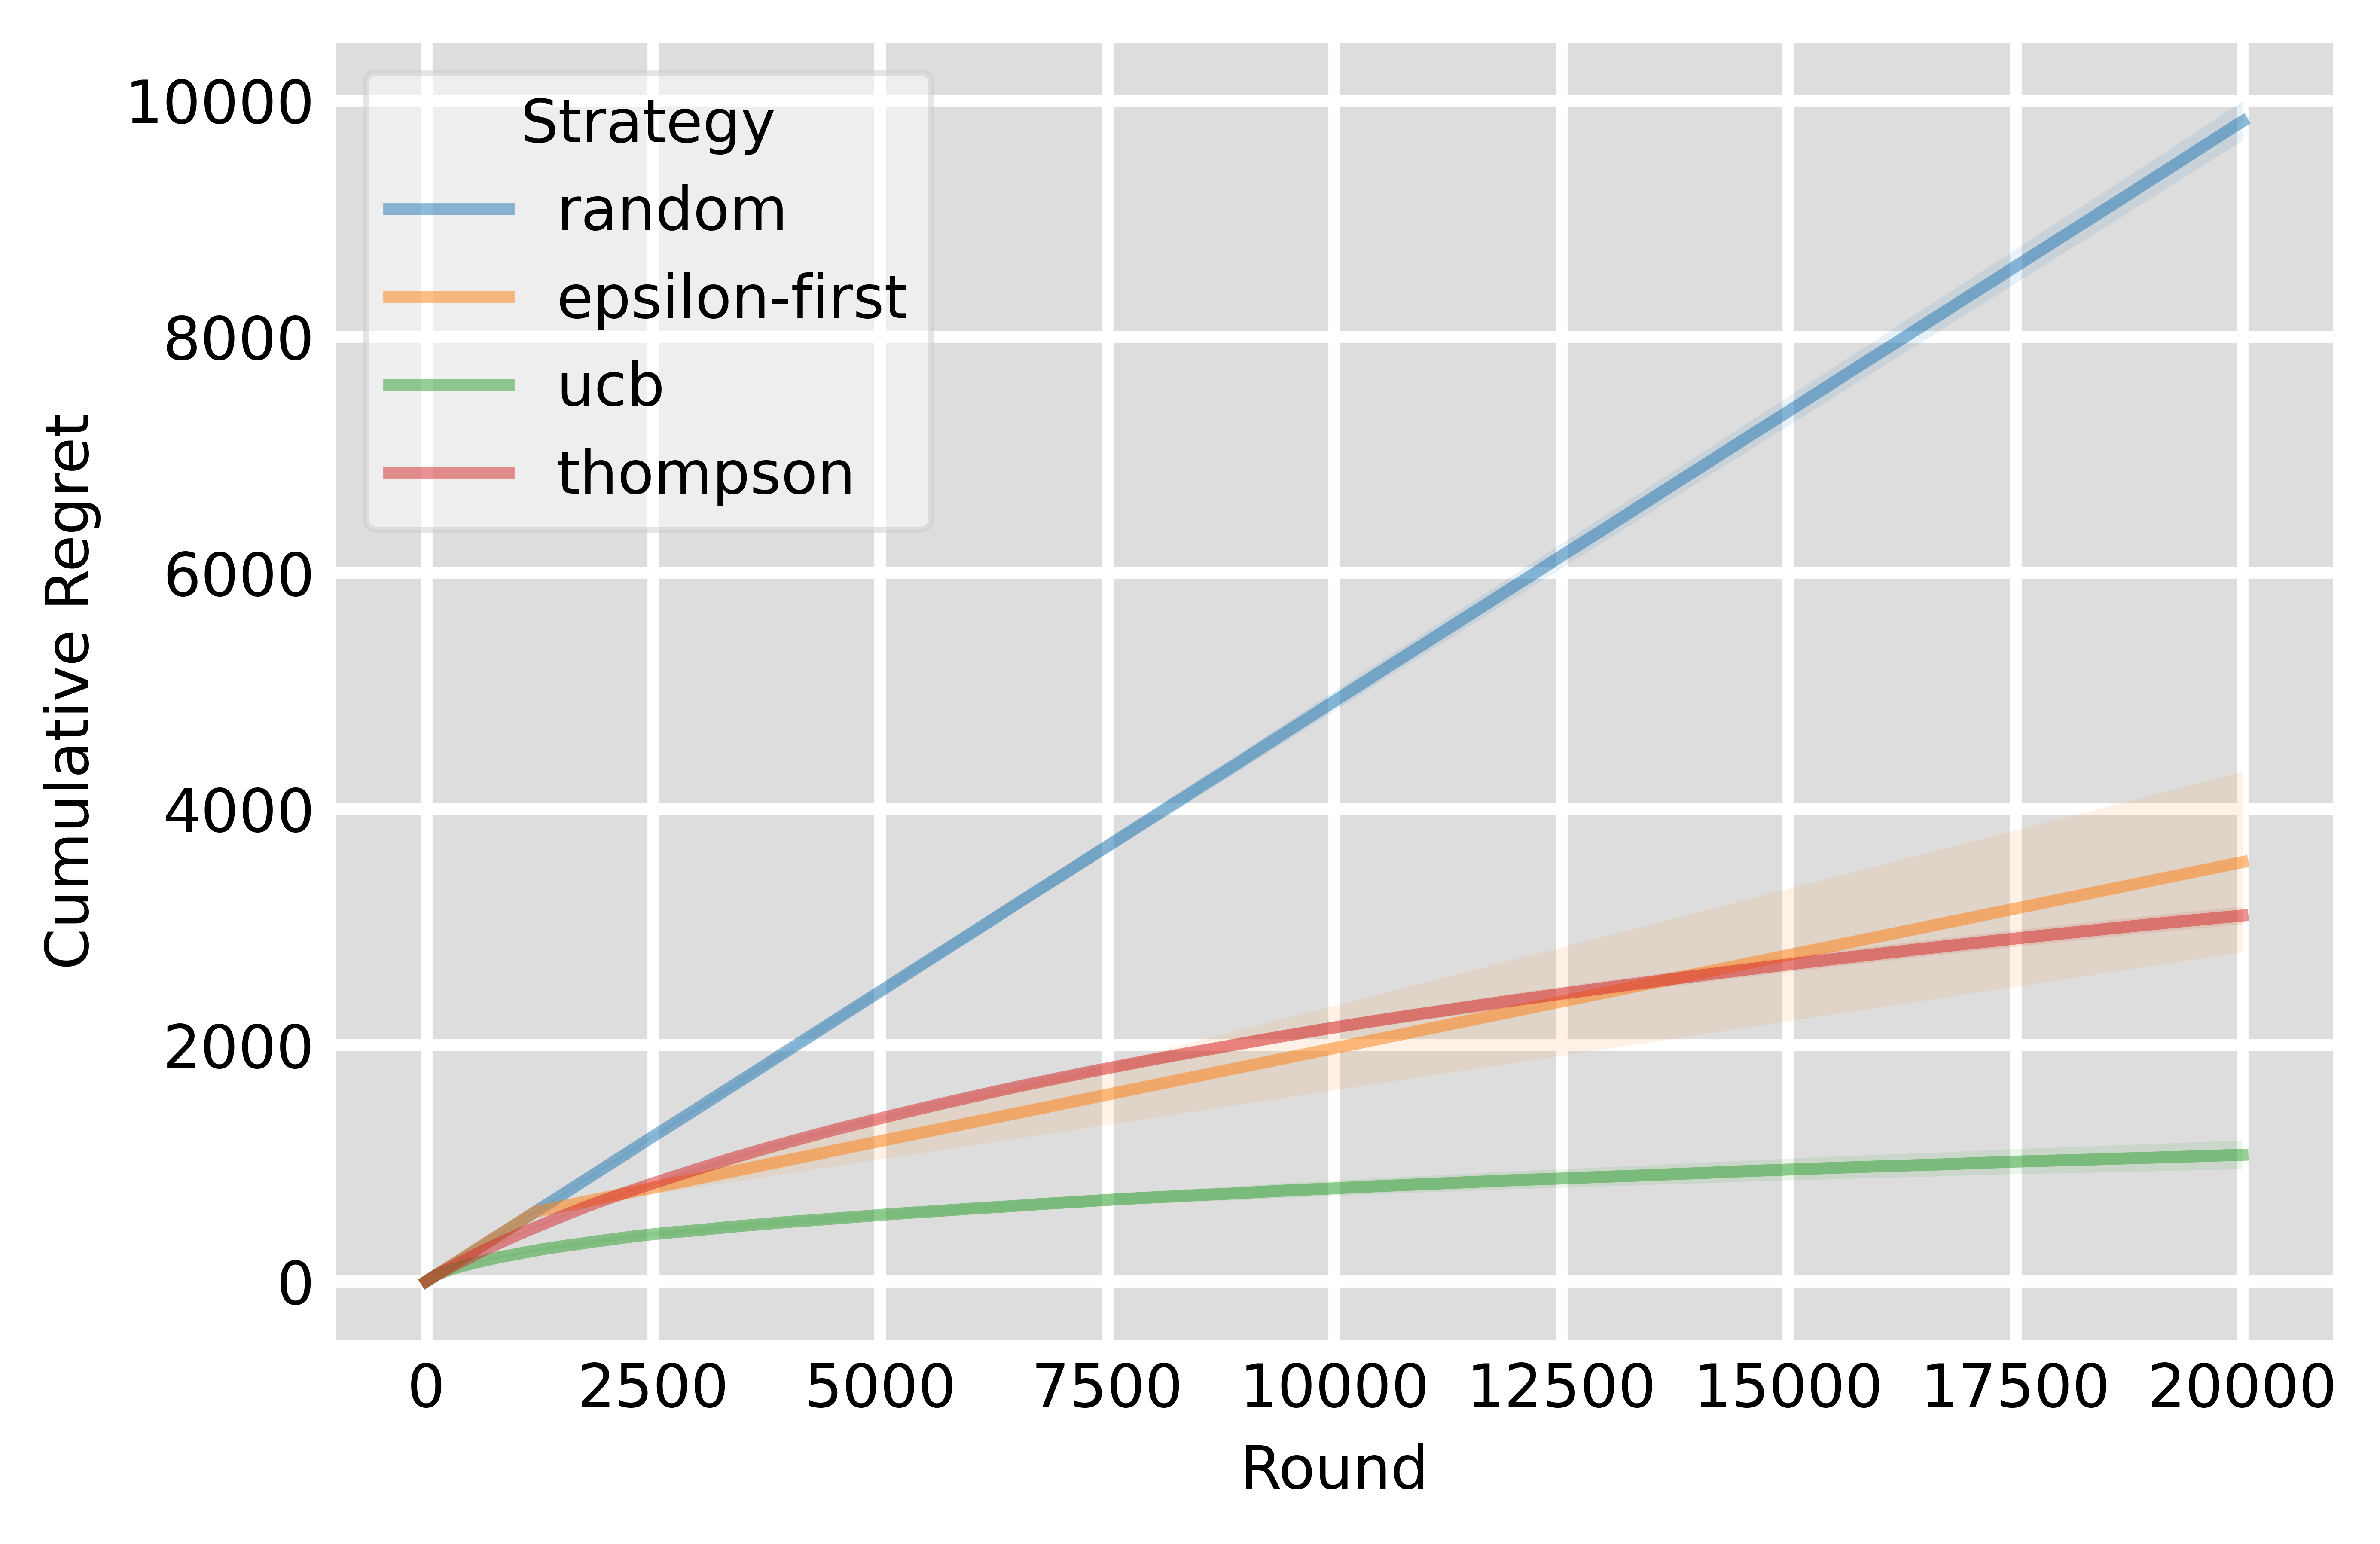
\includegraphics[width=0.9\textwidth]{figures/comparison_of_all_strategies_100_machines}
    \caption[Comparison of Stationary Strategies]{Comparison of Stationary Strategies. Epsilon =0.06, confidence level=1. 100 machines. 20000 rounds per iteration. Average of 50 iterations}
    \label{fig: all1}
\end{figure}

\begin{figure}[h]
    \centering
    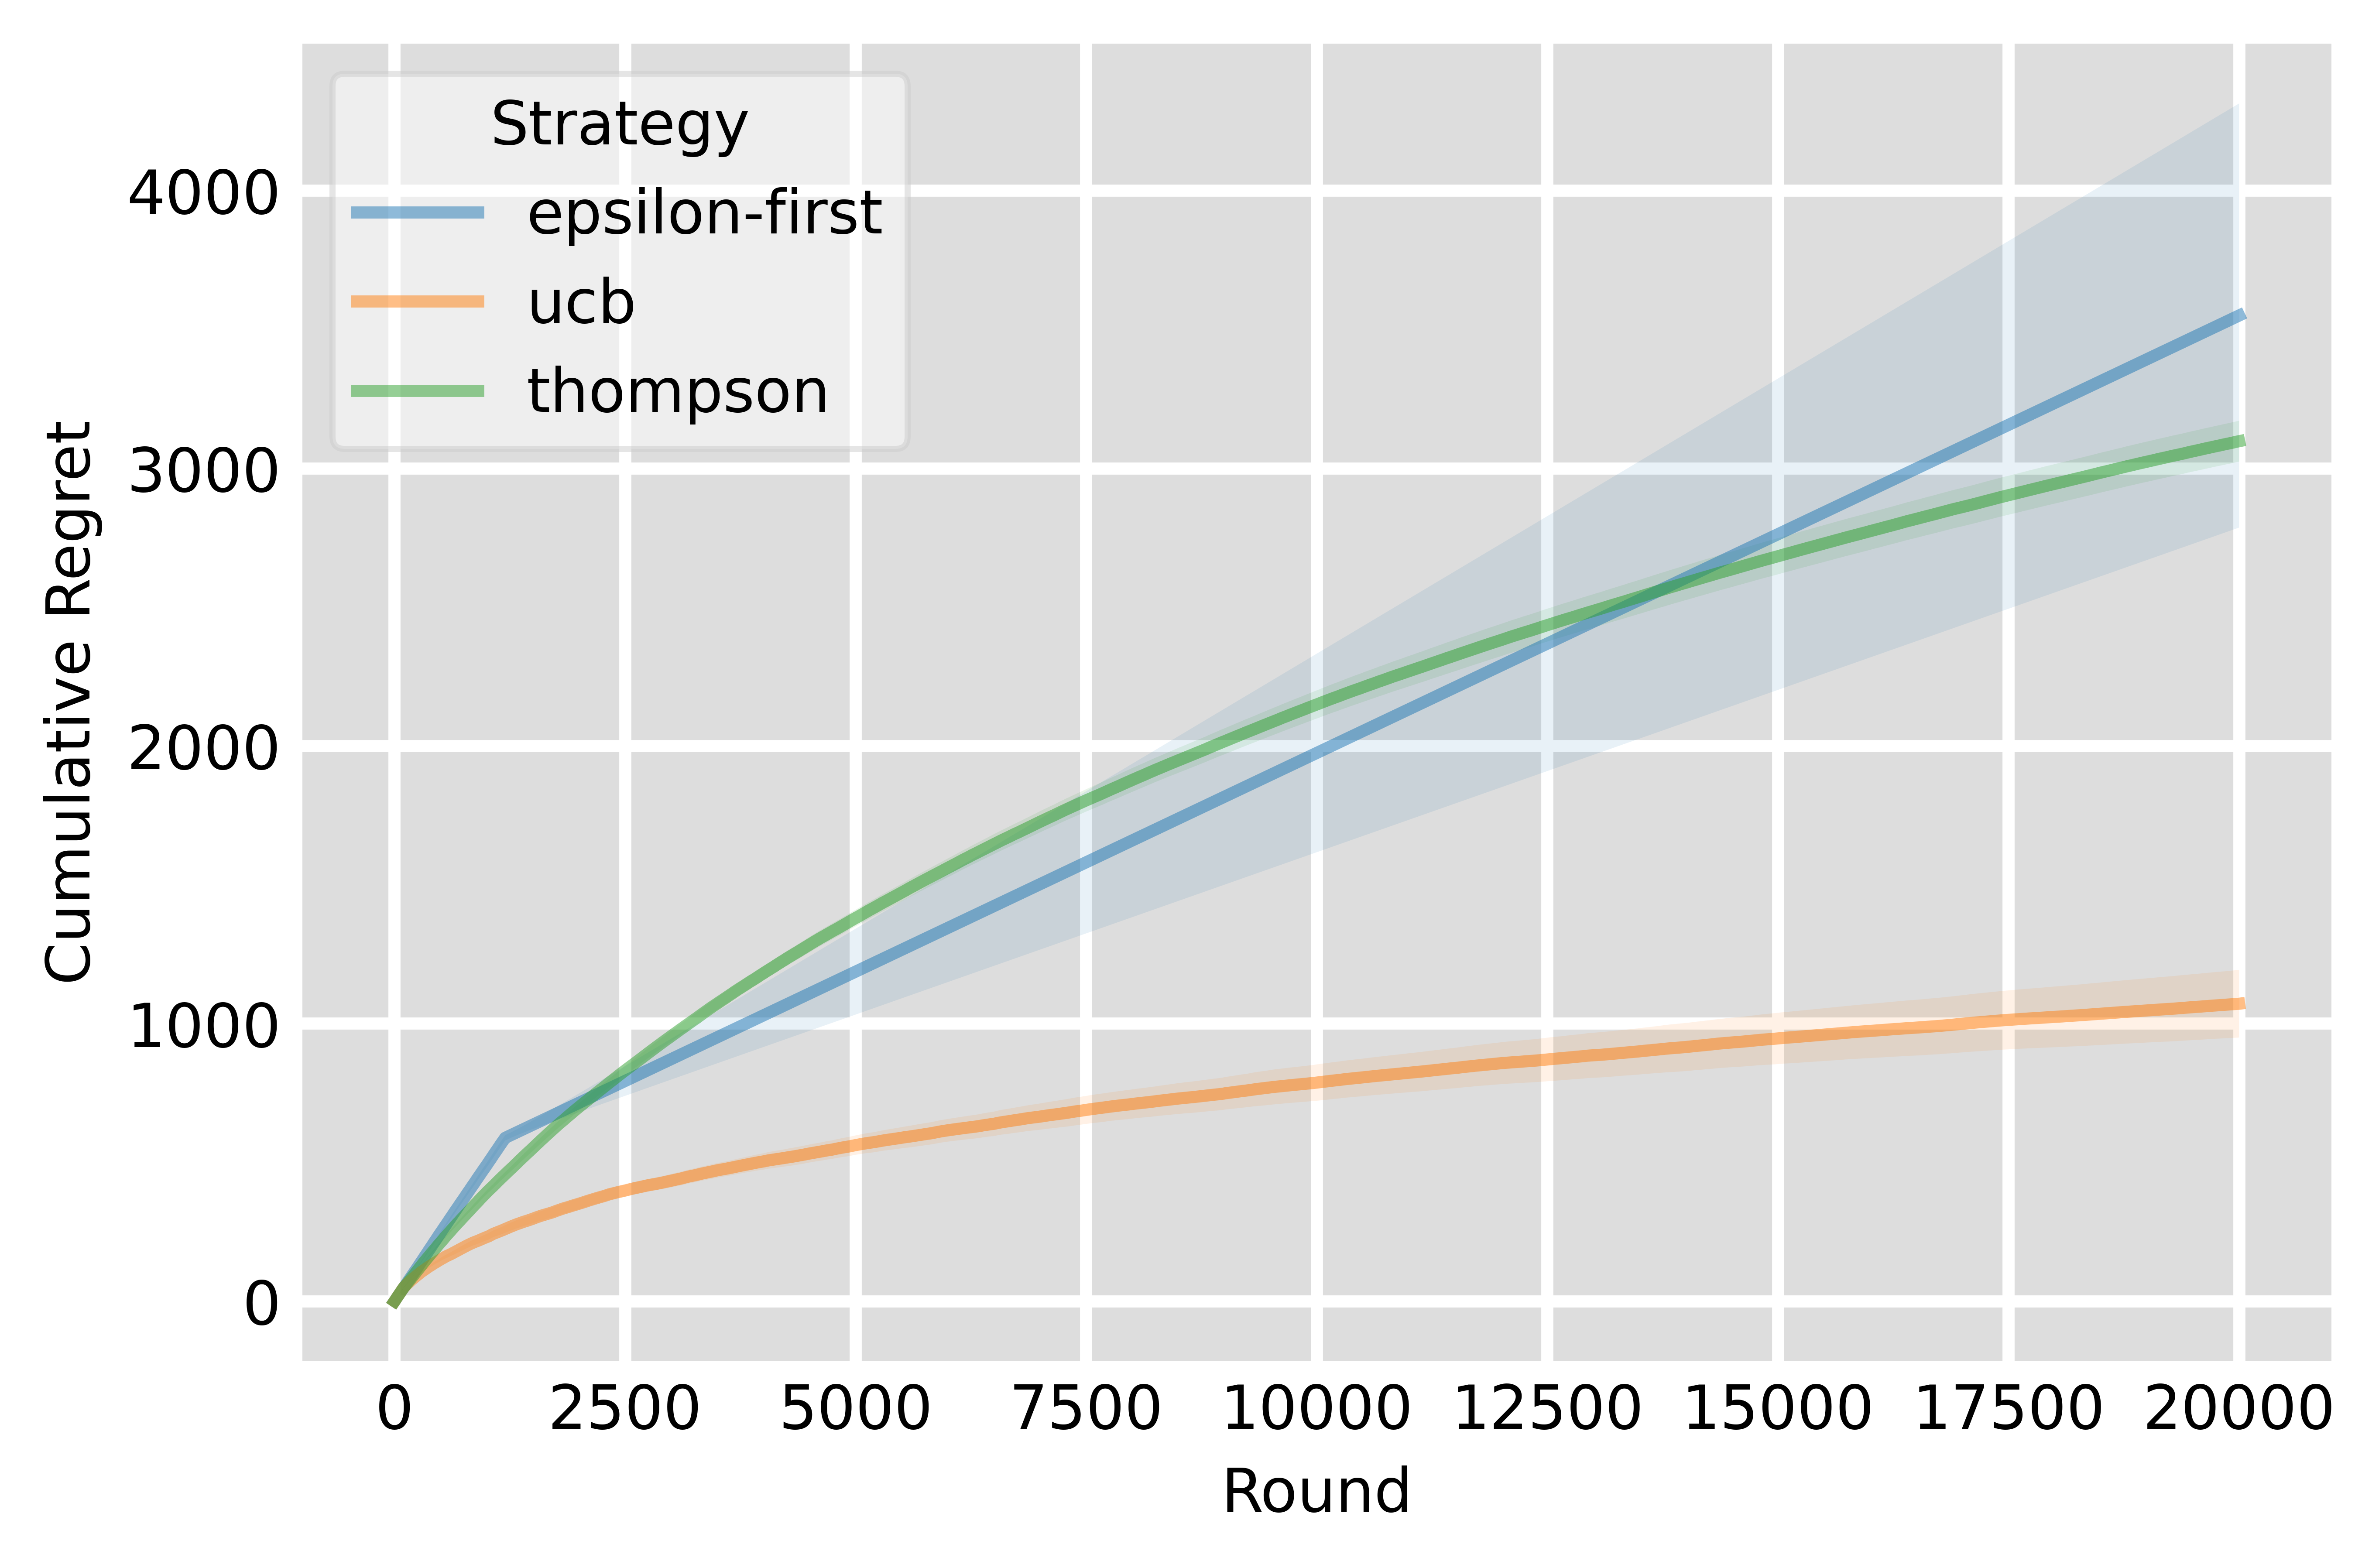
\includegraphics[width=0.9\textwidth]{figures/comparison_without_random_100_machines}
    \caption[Comparison of Stationary Strategies without random]{Comparison of Stationary Strategies without random. Epsilon =0.06, confidence level=1. 100 machines. 20000 rounds per iteration. Average of 50 iterations}
    \label{fig: 100 machines without random}
\end{figure}

\begin{figure}[h]
    \centering
    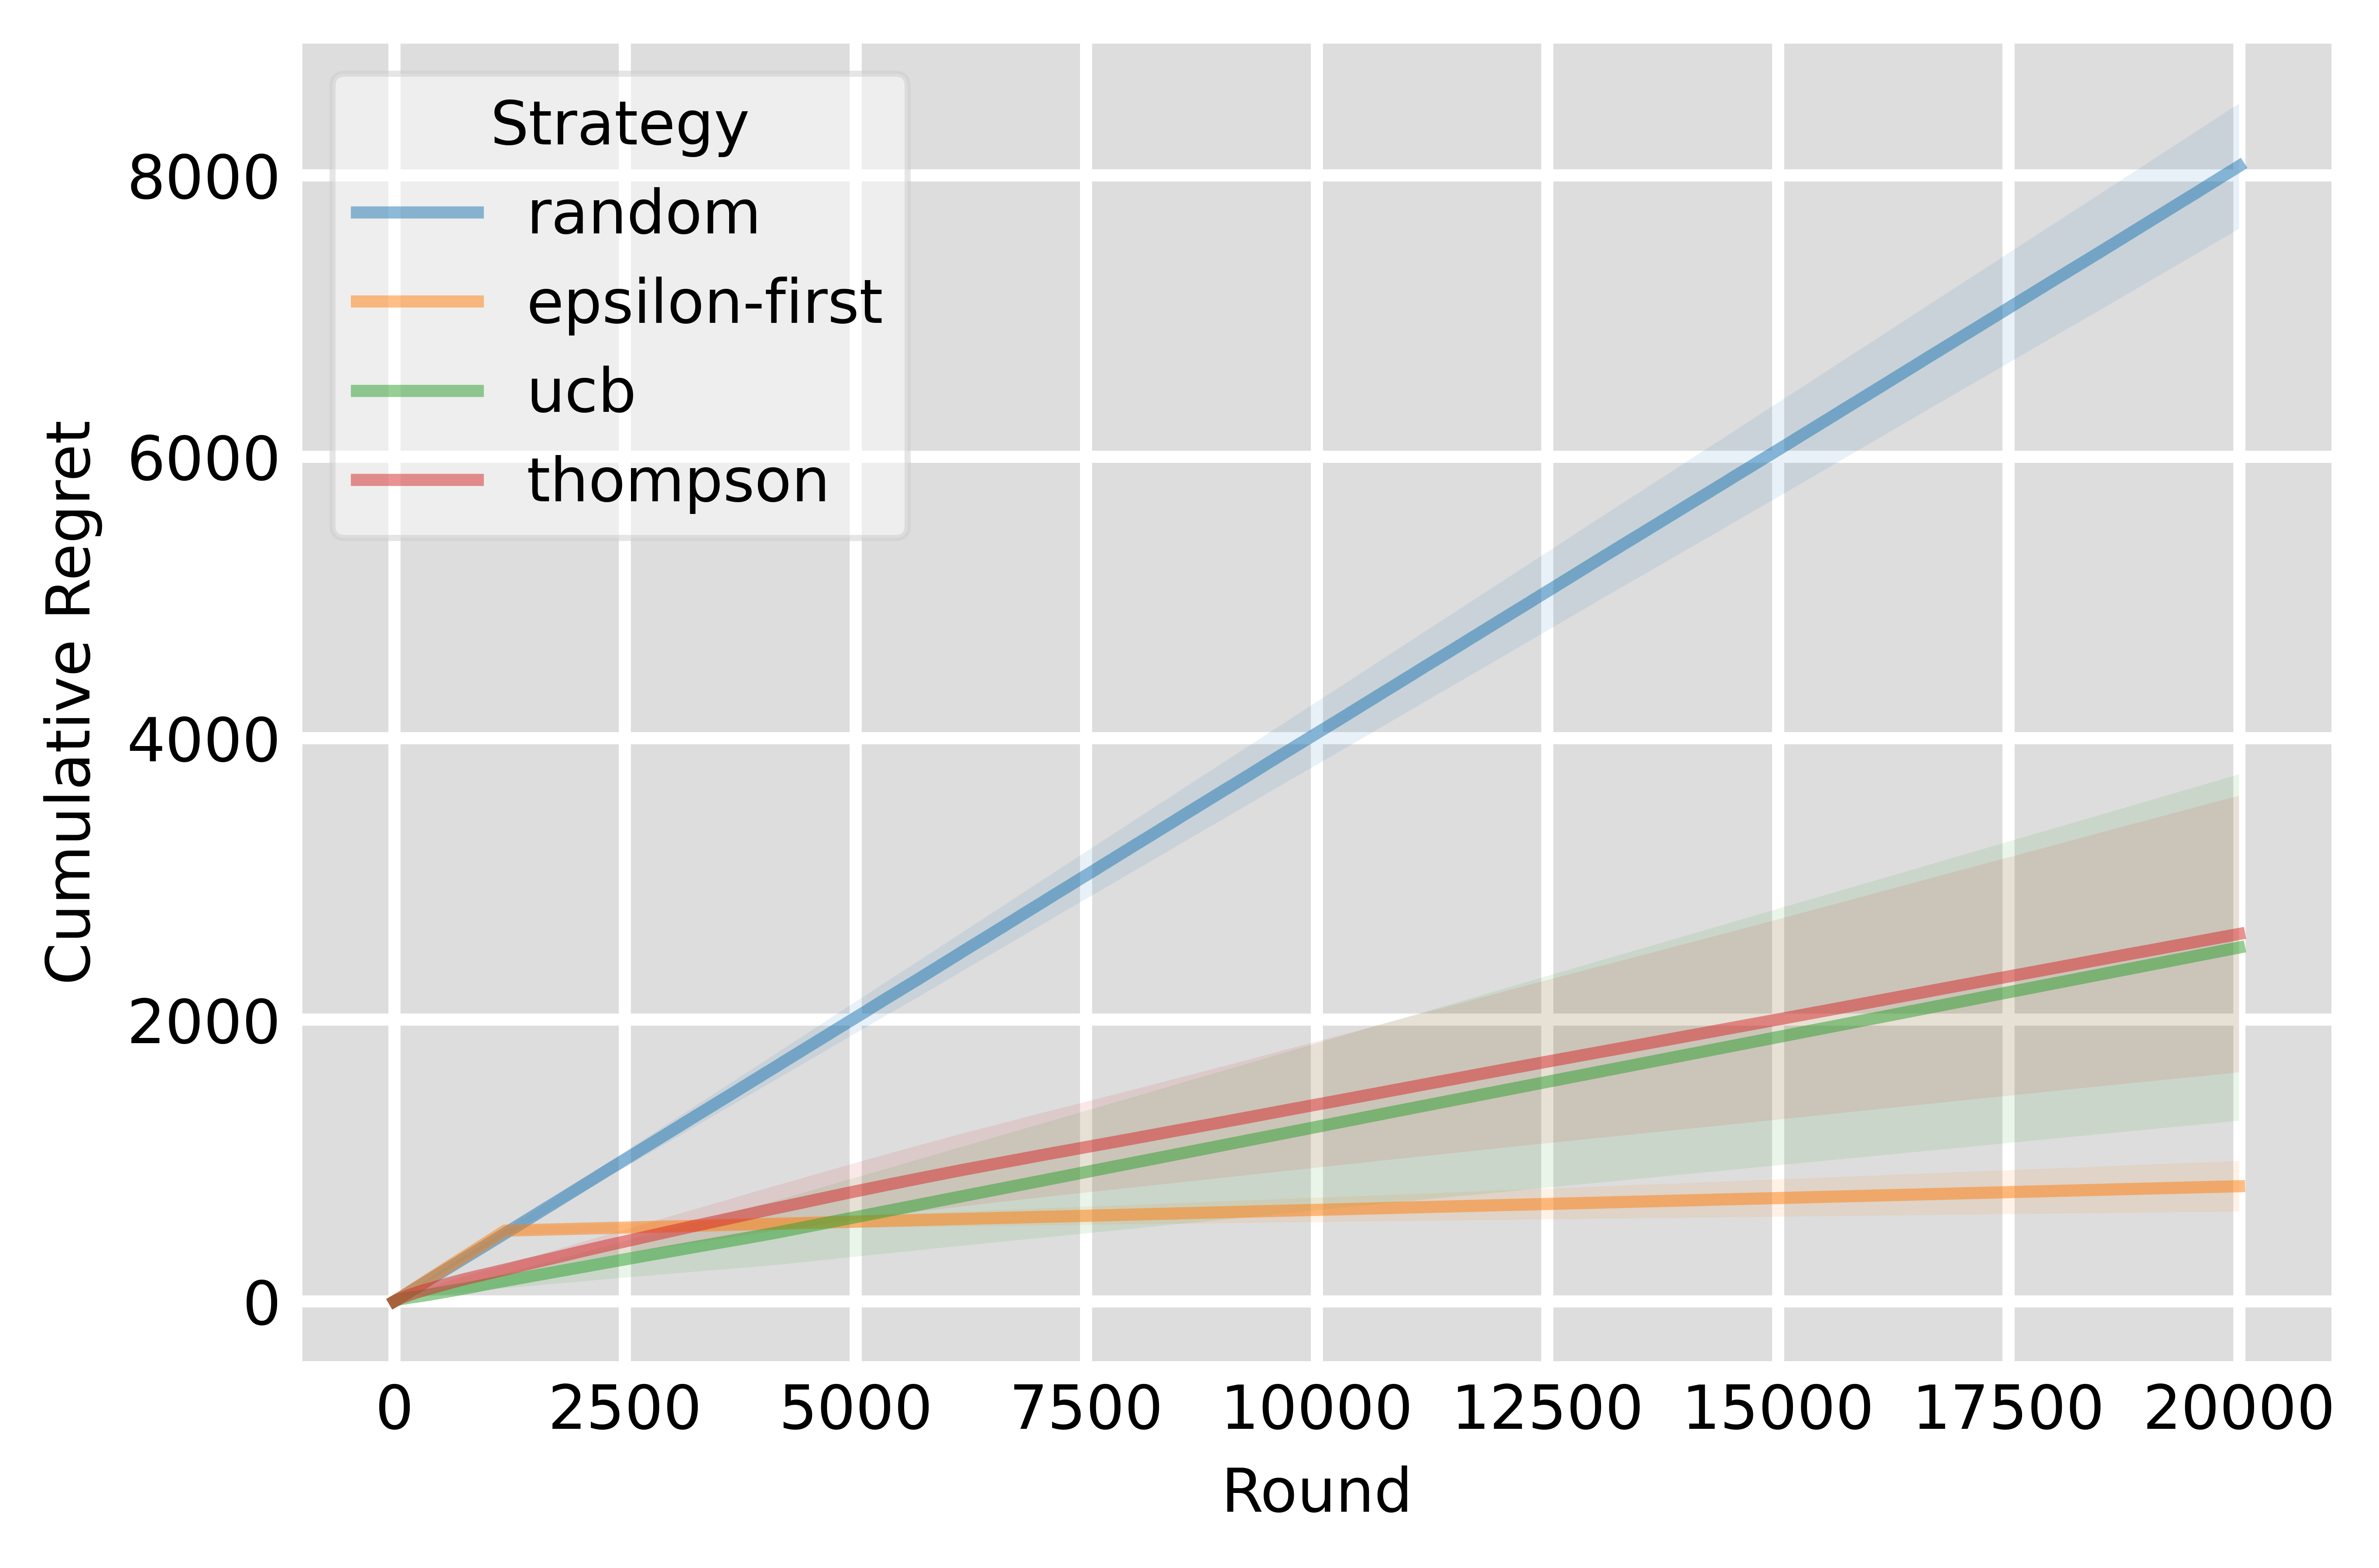
\includegraphics[width=0.8\textwidth]{figures/comparison_of_all_strategies_10_machines}
    \caption[Comparison for 10 machines]{Comparison of Stationary Strategies. Epsilon =0.06, confidence level=1. 10 machines. 20000 rounds per iteration. Average of 50 iterations}
    \label{fig: 10 machines all strategies}
\end{figure}

\begin{figure}[h]
    \centering
    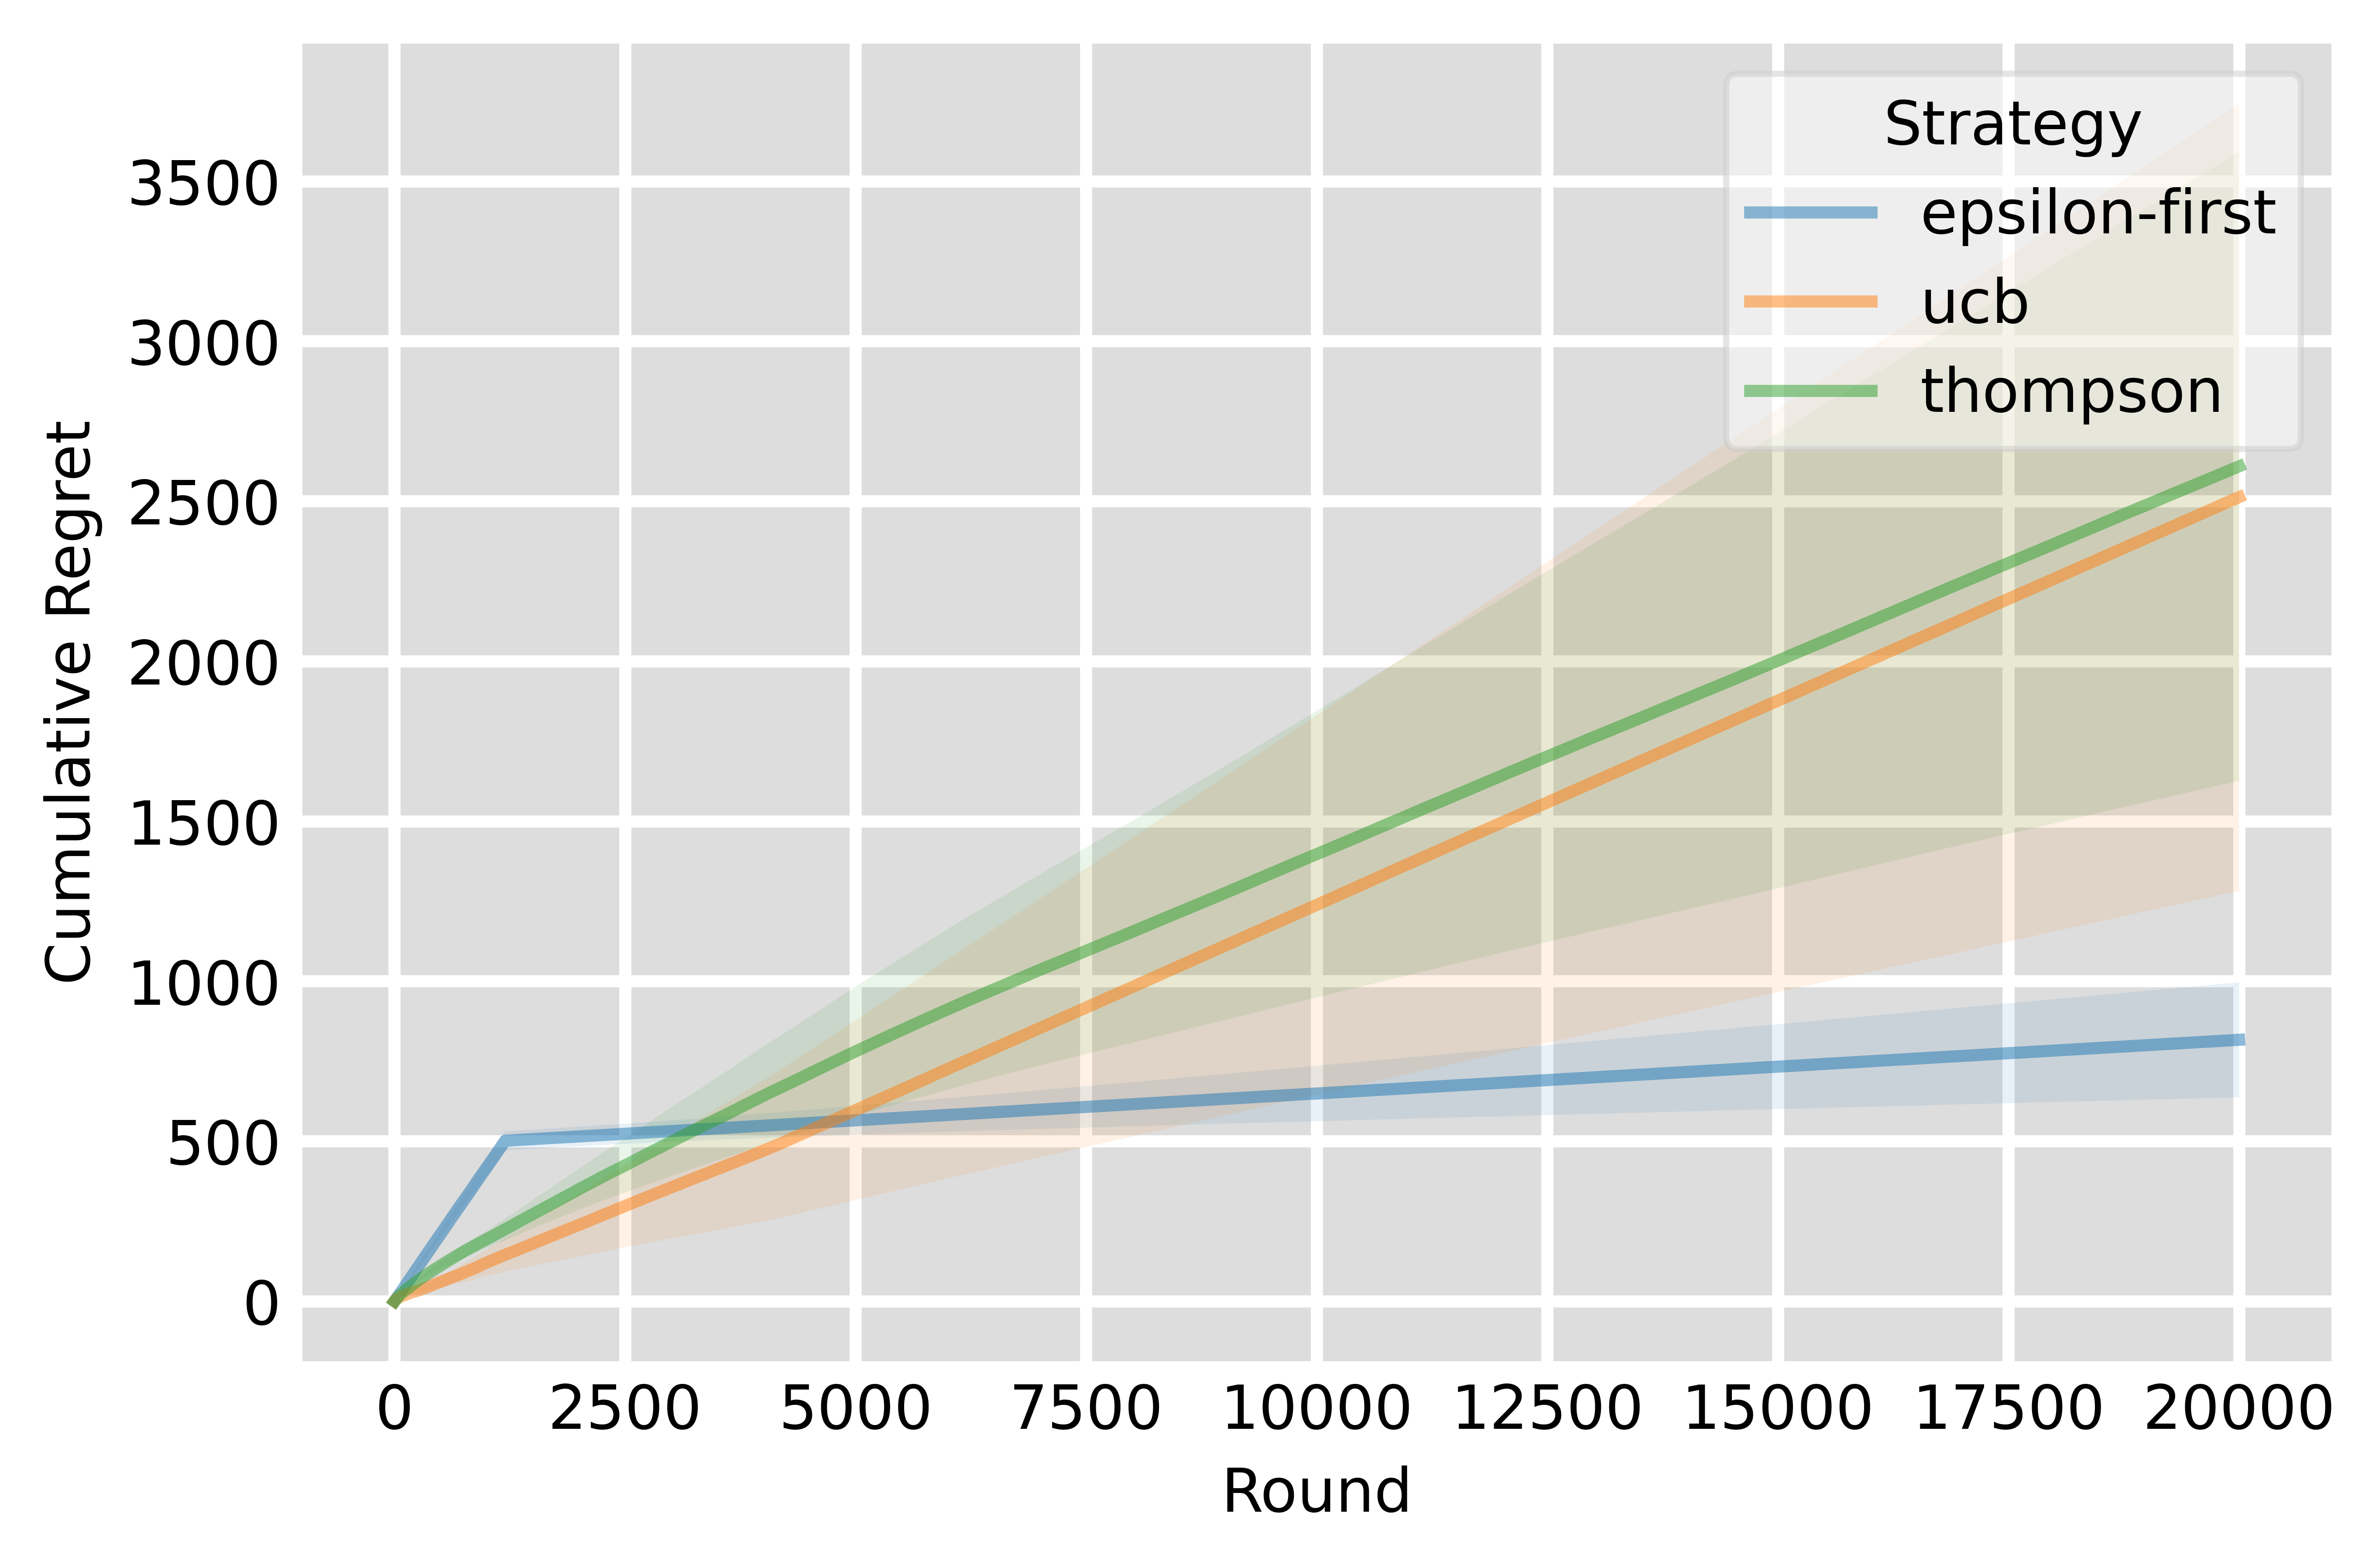
\includegraphics[width=0.8\textwidth]{figures/comaprison_without_random_10_machines}
    \caption[Comparison for 10 machines]{Comparison of Stationary Strategies excluding random strategy. Epsilon =0.06, confidence level=1. 10 machines. 20000 rounds per iteration. Average of 50 iterations}
    \label{fig: 10 machine without random}
\end{figure}

\begin{figure}[h]
    \centering
    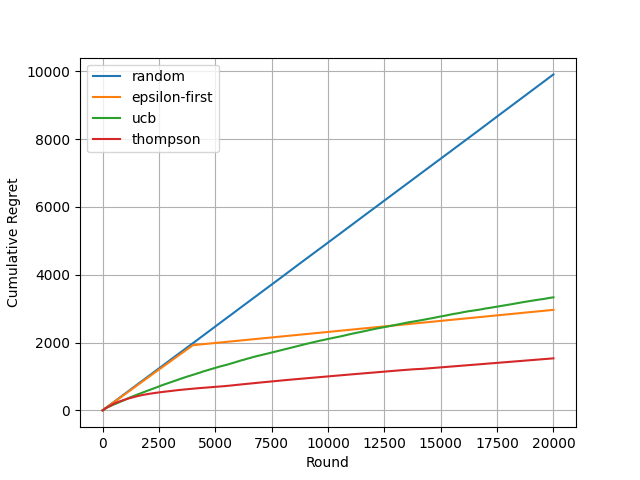
\includegraphics[width=0.9\textwidth]{figures/100machines}
    \caption[Comparison for 100 machines]{Comparison of Stationary Strategies. Epsilon =0.2, confidence level=1. 100 machines. 20000 rounds per iteration. 20 iterations}
    \label{fig: all4}
\end{figure}

We see from above that the $\epsilon$-first strategy isn't necessarily a zero-regret strategy. We see this as the graph for $\epsilon$ = 0.5 doesn't increase in cumulative regret after it finishes its exploration phase, however this is not the case for the two $\epsilon$ values (0.75 and 0.9) which are greater \ref{fig: epsilon}. This demonstrates to us that a higher $\epsilon$ value doesn't mean we are guaranteed to find the arm with the highest actual mean, even with more exploration, due to the fact that we have either had the arm with the highest mean underestimated, or an arm with a lower mean overestimated.

We also see that for our 100 machine plot \ref{fig: all4}, Thompson sampling works the best and is a zero-regret strategy, whilst the random strategy is the worst, with its cumulative regret scaling linearly. Here, UCB also scales to a zero-regret strategy, and $\epsilon$-first does not. However, $\epsilon$-first does better than UCB in the number of trials given, due to a fairly low amount of exploration followed by exploitation ($\epsilon$-value 0.2).